\section{Weyl and 3D Dirac Semimetals}
\label{sec:intro:Weyl}
%1 chiral
%2 from Berry phase to chiral charge
%3 current between the Weyl nodes
%4 poor man�s approach for chiral pumping
%
%experimental progress, ARPES (including Fermi arcs), transport
%
%
%
%Besides the progress in TI, interesting concepts of Weyl semimetals and 3D Dirac semimetals have also been developed.

While the surface states on TI provide an analog to the 2D Dirac electrons in graphene, interesting concepts of Weyl semimetals and 3D Dirac semimetals were also developed as examples of 3D Dirac electrons. With a linear energy-momentum dispersion, both Weyl semimetals and Dirac semimetals can be viewed as 3D analogs of the 2D graphene. Besides, Weyl semimetals provide a solid-state realization of the Weyl fermions that have been studied theoretically for a long time in high energy physics. Weyl fermions are a type of massless fermions with handedness, i.e. chirality. The chirality describes whether a particle spins clockwise or anti-clockwise when viewed in front of the traveling direction. In absence of an electromagnetic field, the chirality of each Weyl fermion is conserved. Therefore, a Weyl fermion cannot shift its handedness without the combination of the electric and magnetic fields. In a 3D crystal, Weyl fermions can be imitated by quasiparticles of electrons with the Hamiltonian as the following:
%\be
%H_{\pm}=\pm \nu_F (p_x \sigma_1 + p_y \sigma_2 + p_z \sigma_3),
%\label{eq:H_W}
%\ee
\be
H=\bf p \cdot \bf V \cdot \pmb{\sigma},
\label{eq:H_W}
\ee
where $\bf V$ is the velocity matrix, $\bf p$ is the electron's 3D momentum vector deduced by the Weyl nodes in the Brillouin zone, and $\pmb{\sigma} = (\sigma_x, \sigma_y, \sigma_z)^T$ denotes the vector formed by the three Pauli matrices. If a Weyl node is at $\bf{k_W}$ in the reciprocal space, then $\bf p= \hbar (\bf k-\bf k_W)$, where $\bf k$ is the electron's wavevector. The Pauli matrices $\sigma_i$ (i = x, y, z) live in the space spanned by the pair of bands that touch at the Weyl nodes. Here each of the two bands is single-degenerate. Thus the system could not respect time reversal and inversion symmetry simultaneously. The above equation shows that the chirality in the Weyl semimetal is formed by the electron's momentum and its peudospin described by the Pauli matrices. Then the chirality of the system is $\chi = sign(det(\bf V))$, which could be $\pm 1$ for the left-handed and right-handed Weyl fermions respectively. As in the case of high-energy Weyl fermions, the Weyl nodes in a crystal always appear in pairs with opposite chiralities. The crystal whose low energy dispersion could be described by Eq.\ref{eq:H_W} near a Weyl node is called a Weyl semimetal.

In addition, we may also have a pictorial understanding of the Weyl nodes and their chiralities from the perspective of the Berry phase. A Bloch 
electron moving inside the Brillouin zone feels the Berry vector potential $\bf A(\bf k) = i \Bra{u(\bf k)}\bf \nabla_{\bf k} \Ket{u(\bf k)}$. This vector potential yields the Berry field $\bf F(\bf k)=\bf \nabla_{\bf k} \times \bf A(\bf k)$ that deflects the direction of Bloch electrons in the momentum 
space. $\bf F(\bf k)$ is also called the Berry curvature or the Chern flux. Thus $\bf F(\bf k)$ acts as a magnetic field that bends the momentum trajectory of a moving electron in a crystal. In a WSM, the chirality $\chi$ of a Weyl node can be calculated by the total Berry flux through an enclosing surface with the following equation:
\be
\frac{1}{2\pi}\oiint\limits_{FS} \VF{F(k)} \cdot \dif{\VF{S(k)}}=\chi, 
\label{eq:chi_Berry}
\ee
where the integral is over the whole Fermi surface that encloses the Weyl node. This equation suggests that a Weyl node acts as a monopole that generates the Berry curvature in the momentum space. Weyl nodes with opposite chiralities are similar to magnetic monopoles with opposite magnetic charges. Besides, since $\bf F(\bf k)$ is the Chern curvature, the above equation indicates that a Fermi pocket that encompasses a Weyl node has a non-trivial Chern number $\chi$.

In a crystal with both time reversal symmetry and inversion symmetry, such separated Weyl pairs do not exist because the bands involved are always degenerate. When two Weyl nodes with opposite chiralities meet in a crystal, they generally annihilate and open a band gap. However, Wang et. al.~\cite{Wang2012, Wang2013}  found that with certain crystal symmetries, paired Weyl nodes can overlap in the momentum space and it results in a new crystal with a linear energy-momentum dispersion, namely a 3D Dirac semimetal. Unlike a WSM, a 3D Dirac crystal respects time reversal and inversion symmetries at the same time. Besides, 3D Dirac cones also accidentally exist in many solids. For example, at the phase transition between a topological insulator and a trivial insulator, the conduction and valence bands of the crystal touch and form a linearly dispersed Dirac cone. However, such accidentally formed Dirac semimetals are not stable since they need fine tuning of chemical compositions and a small perturbation may open a gap at the Dirac point. Nevertheless, the DSMs found by Wang et. al. ~\cite{Wang2012, Wang2013}, i.e. Cd$_3$As$_2$ and Na$_3$Bi, are robust against small perturbations due to the protection by the crystal symmetries. Wang et. al. also predicted the existence of the surface Fermi arcs that connect different Dirac points. Their predictions have been confirmed by ARPES experiments~\cite{Liu2014a, Xu2015, Liu2014, Neupane2014}. Thus such crystals become the maternal materials for Weyl semimetals. Later, Weng et. al. ~\cite{Weng2015} and Huang et. al. group ~\cite{Huang2015} predicted a series of Weyl semimetals that lack inversion symmetry, such as TaAs and NbAs. In these crystals, the Weyl nodes are already separated due to the lack of the inversion symmetry. They also predicted Fermi arcs on the surface that connect the bulk Weyl nodes.Then these findings were confirmed by ARPES experiments~\cite{Xu2015}.

Besides the value in the theoretical aspect, Weyl semimetals also have very interesting transport properties. One of them is the chiral anomaly effect that pumps charges from one Weyl branch to its pair in the presence of an electromagnetic field. A simple picture to understand the chiral anomaly effect in a Weyl semimetal is as the following. If we suppose that the Weyl fermion has entered the lowest Landau level (LL) in a strong magnetic field. The energy dispersion for the $n=0$ Landau level is $\varepsilon_0 = -\chi \hbar \nu_F \VF{k \cdot \hat B}$, where $\hbar$ is the Planck constant and $\VF {\hat B}$ is the normal vector of the magnetic field. We suppose that both the temperature and the chemical potential are low (smaller than $\nu_F \sqrt{\hbar eB}$). Also, the degeneracy of one Landau level formed by one Weyl node is $g = \frac{B S}{h/e}$, where $S$ is the cross-section of the sample that is perpendicular to $\bf B$. If an electric field $\bf E$ is also applied on the same direction as $\bf B$, the states in the momentum space will move according to $\hbar \VF{\dot{k}}=-e  \VF{E}$. Thus the charge pumping rate between Weyl nodes with opposite chiralities is $\VF{\dot{Q}} = e \chi g L |\VF{\dot{k}}|/2\pi=-e^2 \chi g L|\VF{E}|/h$, where L is the length of the crystal along the $\bf B$ direction. Putting in the expression for the degeneracy of the lowest Landau level, we obtain the charge pumping rate for unit volume:
\be
\VF{\dot{Q}}= -\frac{e^3}{4\pi^2\hbar^2} \VF{E} \cdot \VF{B}
\label{eq:chg_pmp}
\ee

%Although we only showed the correctness of the above formula in the case of the lowest LL and when $\bf B$ and $\bf E$ are parallel, strict calculations (cite) have shown that this formula is concrete even more LLs are occupied when $\bf B$ and $\bf E$ are not parallel. 

Although it seems to annhilate or create charges for one Weyl branch, the pumping effect does not violate the charge conservation law in a crystal because Weyl nodes with opposite chiralities always appear in pairs. The above charge pumping effect is also called Adler-Bell-Jackiw chiral anomaly, which was originally used to explain the neutral pion decay in particle physics. Thus the WSM provides us an opportunity to study the chiral anomaly phenomenon in high energy physics.

\begin{figure}[!htbp]
  \begin{center}            
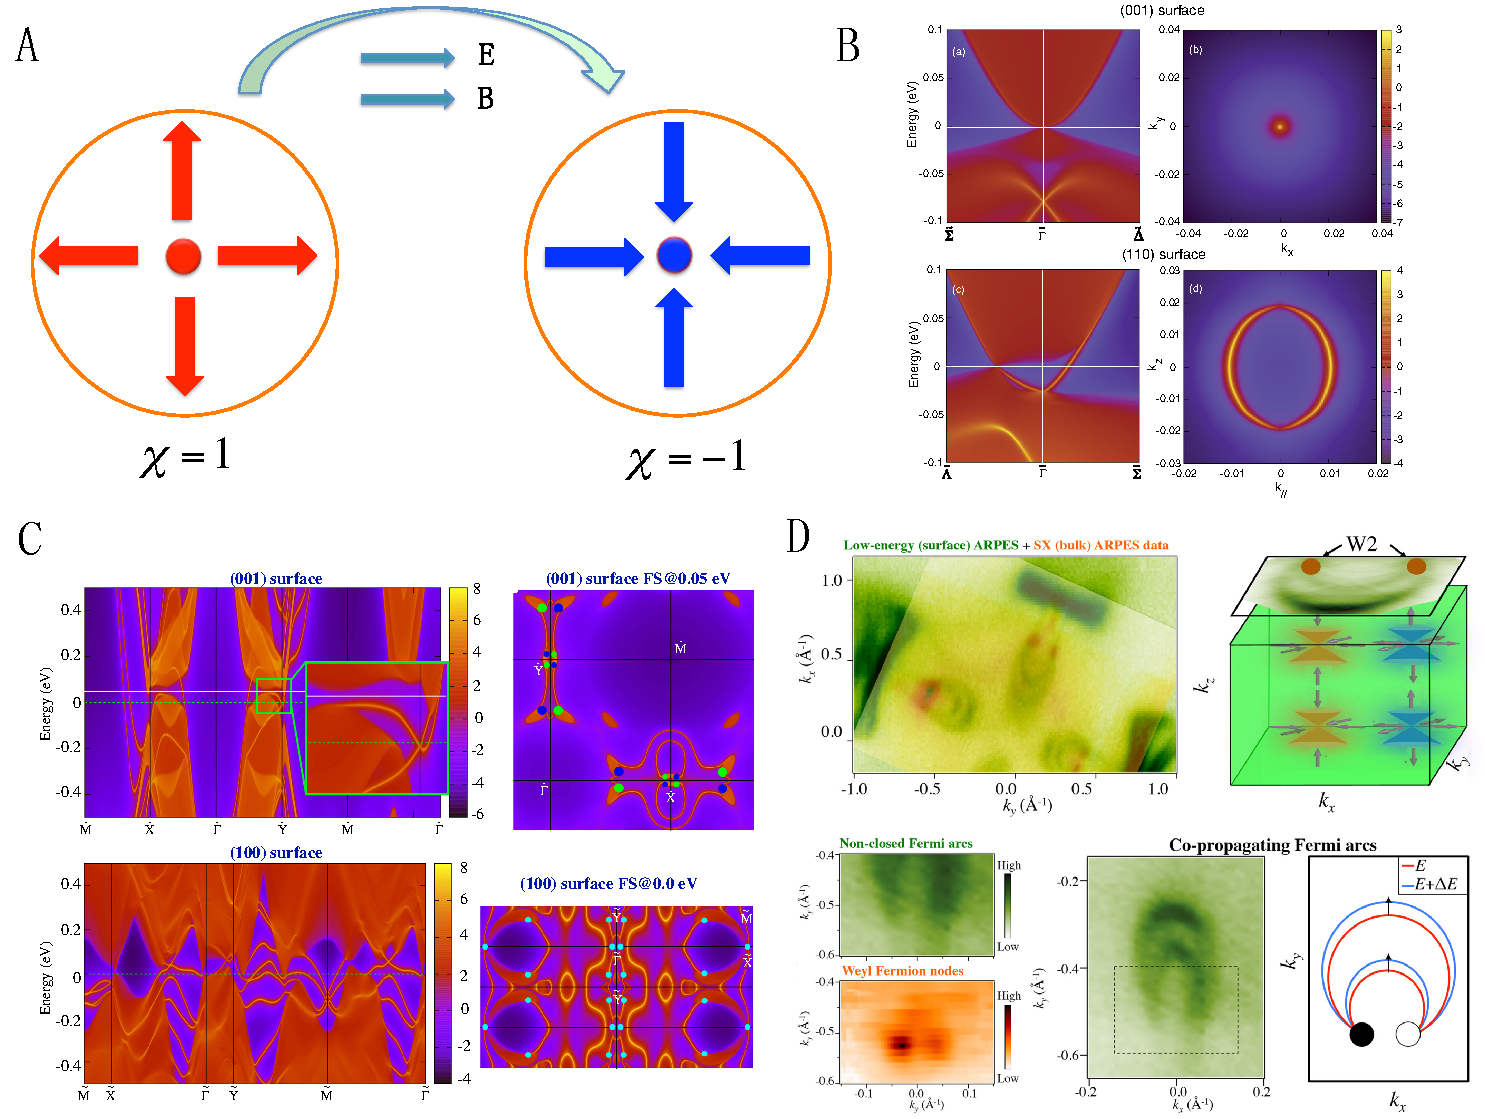
\includegraphics[width=0.9\linewidth]{ch-intro/figures/WeylDirac.pdf} 
\caption{\label{QSHE}
The Weyl and Dirac nodes of Weyl semimetals and Dirac semimetals. (A) The paired Weyl nodes are opposite monopoles of the Berry curvature. In an electric-magnetic field, charges are pumped between the Weyl nodes. (B) The predicted Dirac node and surface Fermi arcs of the Dirac semimetal Cd$_3$As$_2$~\cite{Wang2013}. (C) The predicted multiple Weyl nodes and the surface Fermi arcs that connect them in the Weyl semimetal TaAs~\cite{Weng2015}. (D) ARPES experiments by Hasan's group confirmed the surface Fermi arcs on TaAs~\cite{Xu_TaAs}.
} 
  \end{center}
\end{figure}

